\section*{Aufgabe 20}
\label{sec:Aufgabe2}
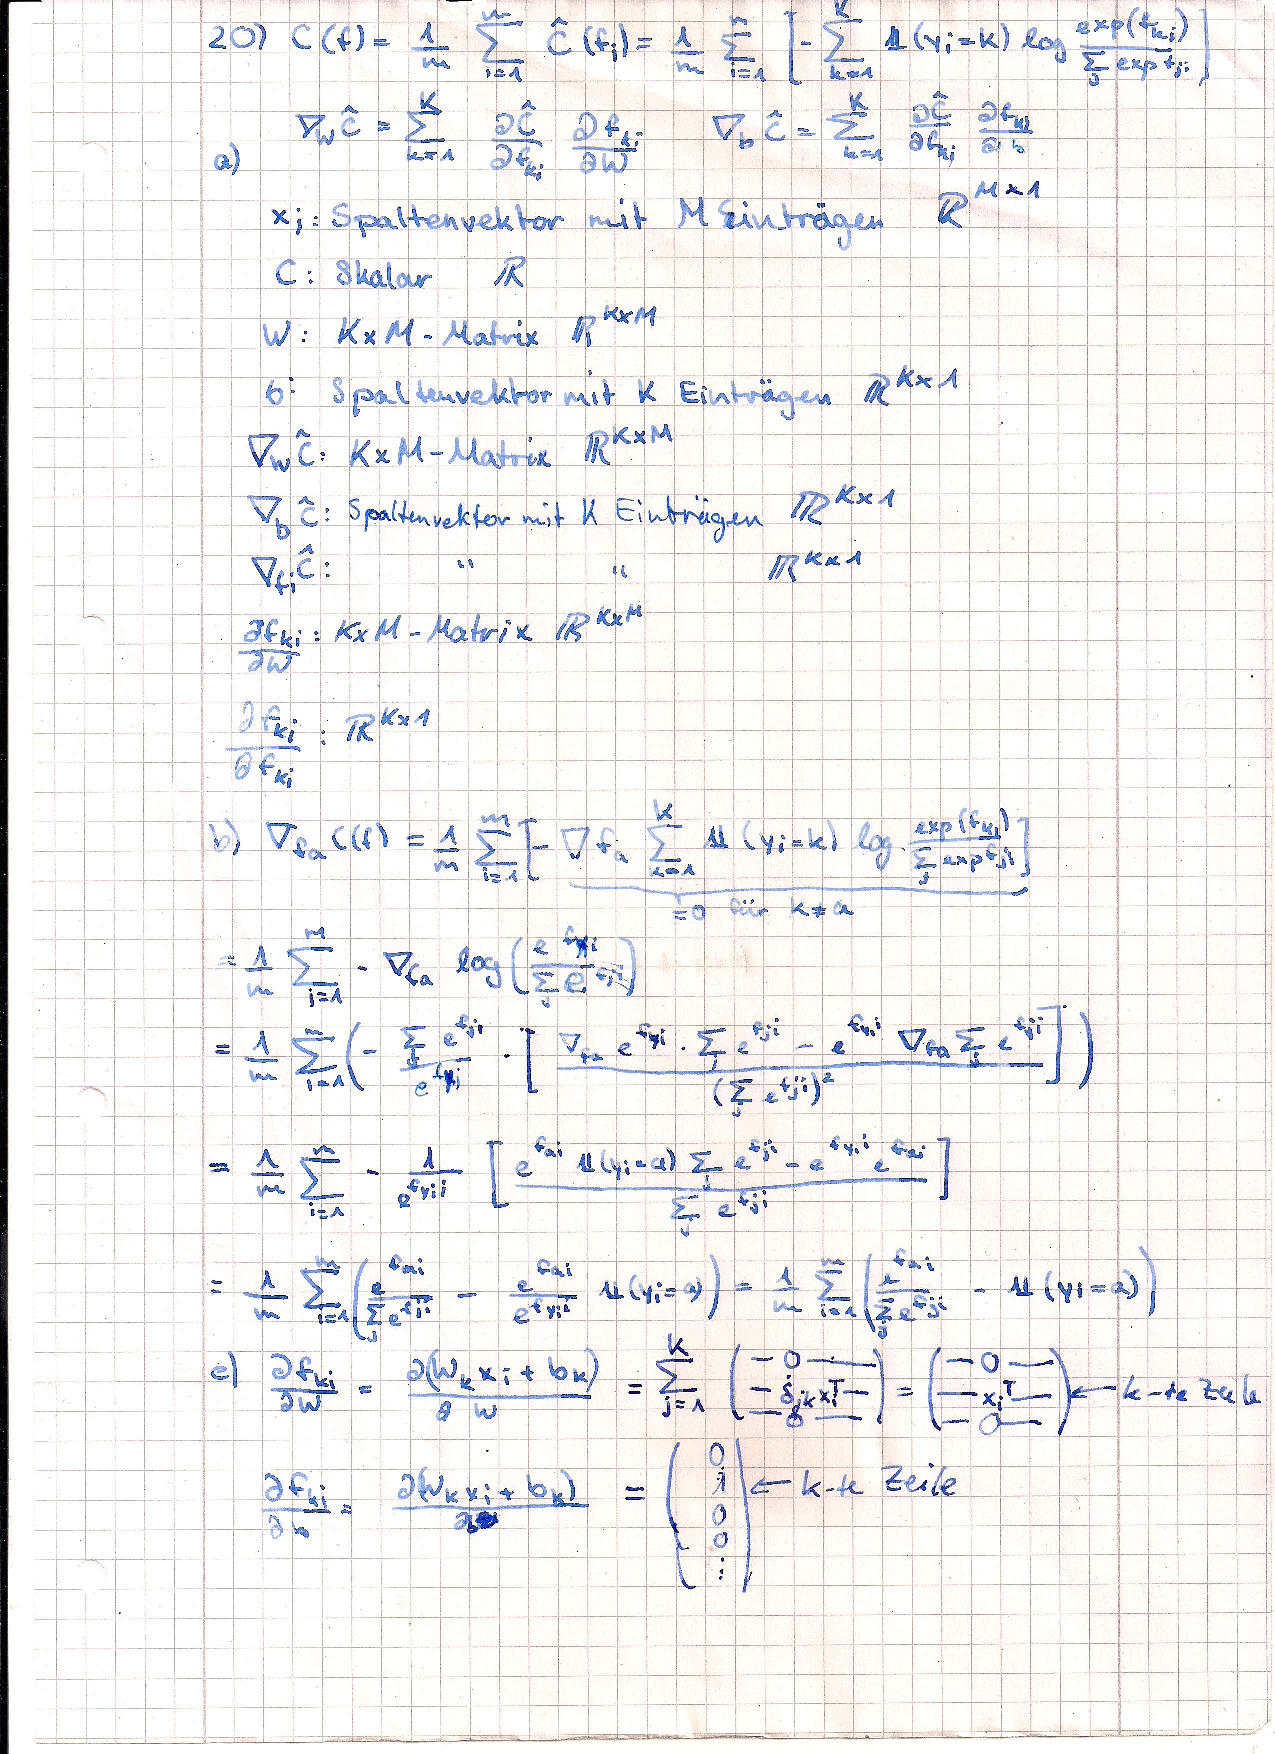
\includepdf[pages=-]{build/20abc.pdf}
\newpage
\subsection*{d)}
In den Zeilen $12$ - $43$ der Python-Datei ist das Training über $100$ Epochen mit einer Schrittweite von $h=0,5$ einer linearen Klassifikation implementiert.
Die resultierende Gewichtungsmatrix ergibt sich zu
\[
W = \begin{matrix}
-1,5569238 & 0,4722979 \\
0,52912648 & -1,94333693 \\
\end{matrix}
\]
und der Bias-Vektor zu
\[
b = \begin{matrix}
-0,23030678 \\
0,974467 \\
\end{matrix}\text{.}
\]
Es zeigt sich, dass das Ergebnis und damit auch die in Abbildung \ref{fig:ger} zu sehende Gerade, sehr stark von den Initialisierungswerten abhängt.

\subsection*{e)}
Der in der Python-Datei in den Zeilen $47$ - $58$ erzeugte Plot der beiden Populationen und der errechneten trennenden Gerade ist in Abbildung \ref{fig:ger} zu sehen.
Die Geradengleichung lässt sich mit der Bedingung $f_\text{1}=f_\text{2}$
und der Gleichung
\[
  \begin{pmatrix}
    W_{11} & W_{12} \\
    W_{21} & W_{22} \\
  \end{pmatrix}
  \cdot
  \begin{pmatrix}
    x \\
    y \\
  \end{pmatrix}
   +
  \begin{pmatrix}
    b_1 \\
    b_2 \\
  \end{pmatrix}
   =
  \begin{pmatrix}
    f_1 \\
    f_2 \\
  \end{pmatrix}
\]
berechnen zu 
\[
y(x)=\frac{b_2-b_1+ x \cdot (W_{21}-W_{11})}{W_{12}-W_{22}}
\]

Der Ansatz $f_\text{1}=f_\text{2}$ bedeutet, dass für die Zuordnung zu beiden Klassen die confidence gleich ist, also die Punkte keiner der beiden Populationen eindeutig zugeordnet werden können.
Dies ist am Übergang zwischen P0 und P1 der Fall, welche für diese Punkteverteilung durch eine Gerade beschrieben werden kann.

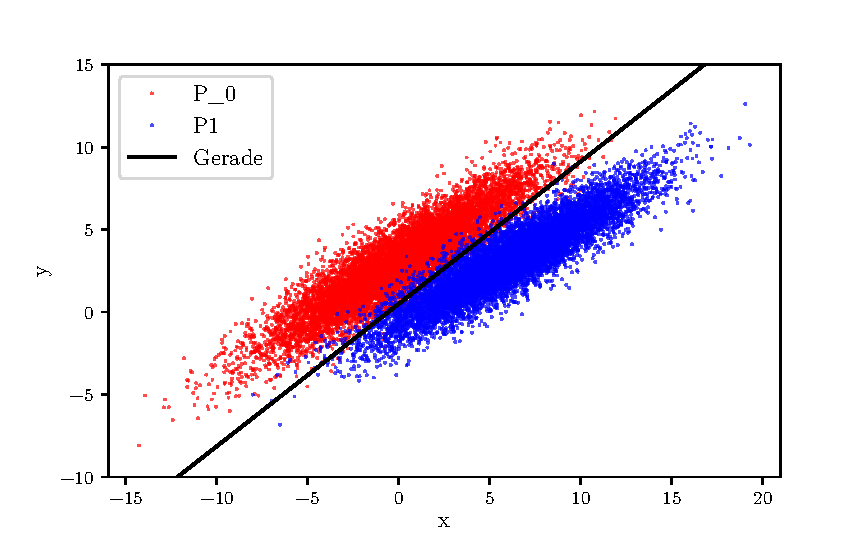
\includegraphics[width=0.8\textwidth]{build/Trennung.pdf}